\documentclass[12pt,letterpaper]{article}
\usepackage{graphicx}
\usepackage{multirow}
\usepackage{authblk}
\usepackage{float}
\usepackage{rotating}
\usepackage{url}
\usepackage{lscape}
\usepackage{longtable}
\usepackage{subfig}
\usepackage{natbib}
\usepackage{lineno}
%\usepackage{fullpage}
\usepackage{anysize}
\marginsize{1.0in}{1.0in}{1.0in}{1.0in}
\linespread{1.6}

\newcommand{\Pic}[2][0.85]{\begin{center}\includegraphics[width=0.8\textwidth,height=#1\textheight,keepaspectratio]{#2}
 \end{center} }


\title{Effect of digital elevation model on Mohr-Coulomb geophysical flow model output}
\author[1]{ E. R. Stefanescu }
\author[2]{M. Bursik}
\author[1]{A.K. Patra}
\affil[1]{Department of Mechanical and Aerospace Engineering, University at Buffalo, Buffalo, NY 14260}
\affil[2]{Department of Geology, University at Buffalo, Buffalo, NY 14260 }

\date{\today}


\begin{document}
\linenumbers
\maketitle

\begin{abstract}
  Digital Elevation Models(DEMs) used in geospatial analysis like the
  simulation of geophysical flows such as floods, landslides and block
  and ash flows, differ in resolution, acquisition time and generation
  methodology, which results in varied representation of topographic
  features. This study investigates the effects of DEMs on the output
  of a granular flow model, TITAN2D by comparing the output using
  different DEMs to that obtained with a "true" representation of the
  terrain, which is considered to be that obtained by using TOPSAR5m
  data. Seven DEMs at four resolutions from four sources were used for
  Mammoth Mountain, California, a cumulodome volcano. TITAN2D was run
  for seven different locations of an eruption of a potential dome and
  two different collapse volumes.  The resulting outputs were
  subsequently compared with TOPSAR5m output, and qualitative and
  statistical inferences were drawn. DEMs with different resolutions
  and sources generated different outputs which led to different flow
  maps. For moderate and smaller scale flows ($\mathcal{O}(10^4)$ 
  $m^3$ -- $\mathcal{O}(10^5)$ $m^3$), different representations
  can affect the computation of accurate footprint of the flow and fine
  DEM resolution is critical for correct characterization of these flows.
\end{abstract}

\section{Introduction}
\subsection{Overview}
The use of computational models to calculate inundation areas by
floods, landslides and volcanic flows is increasing
\citep{Bates2000}. These models depend on proper representation of
topography. Digital elevation models (DEMs) are digital representations of a terrain
 surface and are used to define topographic morphology. 
A DEM is an array of squared cells (pixels) with an elevation associated 
to each pixel. There are different methods  to obtain digital topographic
 data with different levels of accuracy.  The most commonly used 
 methods/instruments are: Shuttle
  Radar Topography Mission (SRTM) interferometry, Advance Spaceborne
  Thermal Emission and Reflection Radiometer (ASTER) digital
  stereophotography, National Elevation Dataset (NED) and LIght
  Detection And Ranging (LiDAR).  The traditional algorithms to obtain
  terrain surface use neighborhood operations to calculate slope,
  aspect and points of inflection \citep{Jenson}. Additional data 
  corrections may include: edge matching, minimizing artefacts or 
  filling of sliver areas of missing data \citep{Zhang2008}.  
  These processes confirm the fact that the
  topographic reality can be represented digitally only to a certain
  level of accuracy.  However, the implicit spatial relationships
  between elevation values can be determined, since the dimensions of
  grid and the number of observations in each row is known \citep{Tate}.
 
 A  common method to obtain a continuous DEM surface from
 contour lines or scattered point elevations is by interpolation. The interpolation
 technique plays an important role in achieving a high accuracy of DEM
 and the choice of interpolation technique depends on the type of
 topography and the distribution of the sample points \citep{Xiao2010, Binh2008}
 
Although DEMs are extensively used in geologic mapping, civil engineering, landscape
planning, visibility analysis, hydrology and geophysical modeling,
and are critical to many natural hazard risk applications, little work has been 
done on the effect of topographic representation
(point spacing, method of construction,etc.) on model output.
 Past analyses generally included a comparison
of numerical model output for digital elevation models (DEMs) created
with the same technology but at different resolution, due to the
limited number of available technologies to create DEMs.    
 \citet{Zhang1994} focused on the effect of DEM grid
size (2m, 4m, 10m, 30m and 90m) on landscape representation and
hydrological modelling with TOPMODEL. Their analysis based on
  variation of the saturation area within a catchment suggested that
10-m resolution data presents a rational compromise between increasing
resolution and data volume for simulating geomorphic and hydrological
processes. \citet{ Wolock1994} evaluated the effect of DEM
 data resolution and map scale on a topographic index, for DEMs in
 eastern Pennsylvania, southern New York, and northern New Jersey.
 The topographic index is a parameter used to characterize
 the topography of a basin. It is defined as $ln(\alpha/\tan \beta)$, where $\alpha$
 is the upslope area per unit contour length and $\tan \beta$ is the local 
 slope angle.
They compared TOPMODEL inputs and outputs calculated with DEMs
digitized from different sources at different resolution (30m and
90m). They concluded that DEMs digitized from higher resolution maps
yield a more detailed representation of topography, but are not
necessarily a better source of topographic information for TOPMODEL
inputs.  They also found out that the mean of the topographic
index distribution increased as data resolution became more coarser.
Another hydrological model \citep{Chanbey2005} for which the effect of
input data resolution was studied was SWAT (Soil and Water Assessment
Tool). Seven secenarios were run at increasing DEM grid sizes (30x30m,
100x100m, 150x150m, 200x200m, 300x300m, 500x500m, 1000x1000m)
on Moores Creek watershed (near Lincoln, AR, USA). Results of
this study indicated that DEM data from 100 to 200 m resolution
achieved less than 10\% error in the model output. In another study,
six DEMs at three resolutions from three sources were used to
calculate the inputs to a soil-erosion model (WEPP )
\citep{Zhang2008}. The study found the 10-m LIDAR DEM to be a
satisfactory input source for the model compared to 30m LIDAR, 4m
LIDAR, 30m NED, 10m NED and 30m SRTM DEM.
\citet{Stevens}investigated the effects of grid-spacing on
  lahar inundation zones predicted by LAHARZ by comparing a 10-m
  gridded DEM with resampled derivatives of 30 m and 90 m
  resolution. No significant effect could be detected except for some
  lahars falling short in travel distance by 1--2 km when using the
  coarser-spaced grids.

Some work has also been done to study the link between ways of
obtaining high-resolution DEMs and the eventual use of the
DEMs. \citet{Cochrane1999} showed that by decreasing the interval
between sampled elevation points, the cost of creating a finer
resolution DEM increases.  Finer resolution DEMs are also commonly
generated from a coarser resolution DEM by interpolation.
\citet{Mitasova1996} used the method of regularized spline
interpolation with tension to create a finer DEM from a 30-m
DEM. However, this method has been criticized by \citet{Zhang1994} and
\citet{Desmet1997} perhaps because it performs poorly when the
  appropriate parameters are not selected.  \citet{Wise2007} created
high resolution DEMs using different methods to run the hydrological
model TOPMODEL. He found that although the total flow, which mostly
consisted of groundwater flow, was little affected by creation method,
the characteristics of the surface flow component were very sensitive
to creation method.
 
There is interest in developing computational models that simulate the
propagation of granular flows such as pyroclastic flows and
rockslide-avalanches as well as the propagation of water.  For such
hazards related models, it is furthermore often important to calculate
inundation areas of the flows under consideration. The TITAN2D model
\citep{Patra2005} performs dry granular flow simulations on a DEM of a
user-define region. DEMs used as TITAN2D input consist of files
containing large numbers of measurements representing the height of
the surface of the earth. These DEMs are obtained using spaceborne,
airborne and photogrammetric elevation data products, such as SRTM,
ASTER, TOPSAR and NED.
In a recent paper,  \citep{Capra2011}  explore the impact of  
topographic resolution alone on TITAN2D simulations of debris flow/
pyroclastic density currents.  Different DEMs of Colima volcano (Mexico)
 at different cell sizes (5, 10, 30, 50, and 90 m) were explored. They performed a qualitative analysis
of  the  velocity and planview trajectories of the flow centerlines, and concluded
that several high resolution DEMs give similar results, while coarser DEM results
are largely different and inaccurate. In this paper we perform a thorough quantitative analysis  of
TITAN2D output to investigate the effects of different DEMs on flow height and flow inundation area calculations.

\subsection{DEM sources and methods of interpolation}
The SRTM (Shuttle Radar Topography Mission) was the first space-borne,
fixed-baseline interferometric synthetic aperture radar (InSAR). In
2000, the SRTM collected interferometric radar data over 80 \% of the
Earth's land surface \citep{Zhang2008}, using a dual-radar
antenna. The goal of a radar interferometer is to measure the
difference in range between two observations of a given ground point
with sufficient accuracy to allow topographic reconstruction. The SRTM
1-arc second DEM ($\sim 30 \times 30$m) represents the raw form of the
SRTM DEM and has a higher resolution than its derivative, the SRTM
3-arc second DEM ($\sim 90 \times 90$m).  For the SRTM 1-arc second
dataset the mission planners anticipated linear vertical absolute
height error to be less than 16m, linear vertical relative height
error less than 10m, circular absolute geolocation error less than 20
m and circular relative geolocation error less than 15 m. These
accuracies were achieved at 90 \% confidence level, consistent with
the National Map Accuracy Standards (NMAS) \citep{Farr2007}.
 
ASTER (Advance Spaceborne Thermal Emission and Reflection Radiometer)
on board the Terra spacecraft is a multispectral optical sensor that
provides imagery with visible and near-infrared (VNIR) bands in 15-m
spatial resolution, shortwave infrared (SWIR) and thermal infrared
(TIR) bands with 30-m and 90-m resolution, respectively
\citep{Abrams2000}. The ASTER instrument produces two types of Level-1
data --- Level-1 A and Level-1 B \citep{Fujisada2005}. Level-1 A data
are defined as reconstructed, unprocessed instrument data at full
resolution. Level-1 A data are used as source data to generate DEM
products, because useful instrument geometric parameters and
spacecraft information are included. Level-1 B data are created by
applying the radiometric calibration and geometric correction
coefficients to the Level-1 A data.  Several study results show that
the vertical accuracy of an ASTER DEM approaches 25m
\citep{Fujisada2005}, but in areas with less vegetation cover, the
accuracy can rise to 9--11m \citep{Goncalves2004}.

The NED (National Elevation Dataset) is a seamless elevation dataset
assembled for the continental US from various data sources. The NED is
a combination of many datasets that consist of digitized USGS
quadrangles, gravimetric surveys, ortho-rectified airphotos, laser
altimeter surveys and SAR surveys \citep{Shaffer2006}.  Available
horizontal resolutions are 10m and 30m.  The USGS creates the original
DEMs by autocorrelation or manual profiling from aerial
photographs. Data corrections are made in the NED assembly process to
minimize artefacts, perform edge matching and fill sliver areas of
missing data.  The NED dataset vertical accuracy is 2.44m RMSE at 90\%
confidence interval according to the NMAS (USGS, 2009).

TOPSAR data are a polarimetric Synthetic Aperture Radar(SAR) dataset
generated by an airborne SAR system \citep{Mouginis-Mark2005}. The
TOPSAR system was implemented via two antennas mounted nearly
vertically on the side of a DC-8 aircraft.  The TOPSAR DEM for our
target area has a resolution of $5 \times 5$m, with a vertical
accuracy of 1.3--2.0 m RMSE \citep{Hooper2003} at 90\% confidence
interval in accordance with the NMAS.
 
 The reason the analysis was
  performed on these particular DEMs was to study model
  characteristics on standard, widely available topographic
  products. NED is the standard topographic model for the US, while SRTM and ASTER are
  widely, almost globally available. It is known that ASTER DEMs
  contain higher vertical errors than SRTM DEMs, while the TOPSAR DEM
  was constructed from high-resolution airborne SAR data with dense
  areal coverage. The TOPSAR DEM is thus little affected by interpolation
  errors, although the data lose accuracy on slopes facing away from
  the sensor, or in areas obscured from the line-of-sight of the
  radar. In many of the above methods of raw data acquisition can result large
  amounts of missing data. This can be caused by the type of relief in the area
  of interest ( e.g SRTM has large amounts of missing data in high relief areas 
  compared to ASTER), around bodies of water and data may be completely 
  missing around areas of persistent cloud cover. We have no information regarding
  the amount of data missing in the raw data or the dates when the data points were collected.
 
 Since elevation data usually consist of discrete, irregularly spaced sample points,
 surface interpolation techniques are used to transform discrete elevation
 data to a DEM surface with regularly spaced data points.  Algorithms to perform the interpolation include techniques such as
 inverse distance weighted (IDW) or bi-cubic spline interpolation, Triangular 
 Irregular Network construction, kriging, finite elements, etc. \citep{Florinsky1998, Cebecauer2002}. Some recommendations 
on choosing interpolation technique were made: for mountainous areas 
 the spline regularized is the most suitable, for gentle hilly and flat 
areas, IDW or kriging are recommended  \citep{Mitasova1993, Binh2008}.  To produce a DEM dataset to which we had ourselves applied a standard interpolating methodology, we calculated a 
30 m DEM obtained from the 5 m TOPSAR DEM using spline interpolation.
\textit{The spline interpolation} estimates the elevation of a specific point using a 
mathematical function that minimizes the overall surface curvature, resulting in a smooth 
surface that passes exactly through the input points \citep{Kamada2009, Xiao2010}.
There are two spline methods: regularized and tension. The regularized method creates a 
smooth, gradually changing surface with values that may lie outside the sample data range. The 
tension method is based on the assumption that the interpolation function should pass through (or
close to) sample points and should be at the same time as smooth as possible \citep{Mitasova1993, 
Kamada2009, Kvasov20011}.
The main parameters of the spline interpolation are the number of 
sampled points used for interpolation, and the 
weight. For the regularized spline, the higher 
the weight, the smoother the output surface. For 
the tension spline, the higher the weight, the 
coarser the output surface.  The parameter values used in a particularly instance of splining are quantitative measures that 
describe only a statistical aspect of interpolation quality, so applicability of
the interpolated DEM for a specific purpose is not known a priori (e.g. correct
representation of undersampled features important to a flow model).

 
Hypothesis tests are usually conducted in all fields in
which theory can be tested agains observations. The null 
hypothesis is a statement that we want to test. In general, the 
null hypothesis is that things are the same, or the same as a 
theoretical expectation.
In this paper, we test the simple hypothesis that different DEMs
result in different model outputs. To test the hypothesis, an
analysis is carried out by comparing the results against the null
hypothesis that different DEMs yield the same model output. 
We furthermore analyze the results to determine if the test outcome is
dependent on flow volume or on the particular DEM used. 
Because it is not possible to have a DEM that represents the ``true'' topography,
the hypothesis is tested using the best DEM available for the area. In
our case, the TOPSAR 5-m DEM is considered the ``truth''. 

This paper focuses on the datasets available for Mammoth Mountain, performing a
qualitative and statistical analysis to address how different the
datasets are in terms of their effect on the computation of granular
flow propagation.


\section{Technical Approach and Methodology}\label{technical}
The TITAN2D code used in this effort conducts numerical simulations of
flows on digital representations of the natural terrain.  It is based
on a depth-averaged model for an incompressible granular material,
governed by Coulomb-type friction interactions \citep{Savage1989}.
The governing equations are obtained by applying conservation laws to
the incompressible continuum, providing appropriate constitutive
modeling assumptions, and then taking advantage of the shallowness of
the flows (flows are much longer and wider than they are deep) to
obtain simpler depth-averaged representations \citep{Patra2005}. The
motion of the material is considered to be gravitationally driven and
resisted by both internal and bed friction forces. The stress boundary
conditions are: no stress at the upper free-surface and a Coulomb-like
friction law imposed at the interface between the material and the
basal surface. Note that the primary factor driving the flow is the
component of gravity along the surface which depends on a local slope
computed from the elevation data.  The resulting hyperbolic system of
equations is solved using a finite-volume scheme with a second-order
Godunov solver. We have thus used a fixed-rheology model, which we agree cannot
  give accurate interpretations or predictions of debris flow motion
  because of their complex behavior, but the Coulomb rheology has
  proven to be a reliable option for coarse solid constituents and
  flow models based on the mechanics of granular media. In a Coulomb
  model the shear stress is a function of a bed friction and/or
  internal friction angle and the effective normal stress, and
  hence is, contrary to rheologic approaches for viscoplastic fluids,
  independent of the shear rate.  Mohr-Coulomb models are used to
  describe 'hard suspension' models, when the frictional interactions
  between particles comprise the dominant process.  'Soft suspensions'
  correspond to viscoplastic flow behavior and phenomenological laws
  like the Bingham or the generalized Herschel-Bulkley for rheological
  behavior.


The program runs in parallel, using the message passing interface
standard (MPI) to allow communication between multiple processors,
increasing computational power, decreasing computational time and
allowing use of large datasets. The algorithm uses local adaptive mesh
refinement for shock capturing, and dynamic load balancing for the
efficient use of computational resources. Topographic data are
included in the simulation by using a preprocessing routine in which
digital elevation data are imported. The DEM file containing X,Y,Z
data (typically UTM easting, UTM northing and elevation in meters)
must be properly configured to operate with TITAN2D through the use of
a header.
The other input parameters for the model which describe the initial 
geometry of the dome and control the flow movement are presented in Table \ref{tab:Table1}.

TITAN2D was run for a few combinations of the parameters that characterized the 
 initial failure (Table \ref{tab:Table2}): two different-sized volumes, and seven
different starting locations. The initial pile shape is a paraboloid
for which the volume is calculated as $V=\frac{\pi}{2}\cdot r_{min}\cdot r_{max} \cdot h_{max}$.

 The study area is Mammoth Mountain --- a large, geologically
  young, composite dome volcano located on the southwestern rim of
  Long Valley Caldera, California \citep{Bailey1989}. The summit ridge
  is composed of 18 domes and/or lava flow units
  \citep{Burkett2007}. The summit itself is 3,371 m above sea level,
  and more than 1,200 m above the general level of the adjacent
  caldera floor \citep{Farrar1995}.  Phreatic eruptions from vents on
  the lower portion of the mountain in 667--737 calBP 
  directly preceded the magmatic 605--625 calBP North Mono eruption
  and the 1350 AD ($= 600$ calBP) Inyo eruption. Recently, an 
  anomalously high level of $CO_2$ has
  been discovered in the local soil and groundwater, suggesting the
  existence of a large mass of free magmatic gases and/or a water
  reservoir beneath Mammoth Mountain saturated with magmatic gases.
  These data taken together suggest that magmatism
  underneath the mountain has been rejuvenated, and that this
  rejuvenation could lead to explosive events, including the
  generation of both pumiceous and dome-collapse pyroclastic flows.

Common hazardous geophysical mass flows on Mammoth Mountain might
contain $O$($10^5 - 10^8$) m$^3$ material \citep{Patra2005,
Burkett2007}. We consider two flows --- a low-volume flow with an
initial volume of $1.54 \times 10^5 m^3$, with a maximum initial
thickness of $h_{max}= 20m$, major axis $r_{max} = 70m$ and minor axis
$r_{min} = 70m $, and a high-volume flow of $2.82 \times 10^7$ m$^3$
corresponding to $h_{max} = 200m$ and $r_{max} = r_{min} = 300m$.  By
using two endmember volumes, we can observe extrema in the effect of
volume on the output for different DEMs.

By choosing seven potential starting locations, we are trying to cover
an area near the summit where we observed that potential vents could
be situated, based on positions of ancient vents \citep{Bailey1989,
Burkett2007} (Figure~\ref{fig1}). The flow maps were constructed by combining
the maximum pile height of the individual flows. In case of an flow overlap
the maximum of the piles height was plotted. The properties of the flowing
material are taken into account by choosing appropriate values for the
bed ($\phi_{bed}$) and internal friction angles ($\phi_{int}$): 20
degrees and 25 degrees, respectively.

The DEM's available for experiment are: TOPSAR ($5 \times 5$m and $30
\times 30$m resolution), NED ($10 \times 10$m and $30 \times 30$m
resolution), SRTM ($30 \times 30$m and $90 \times 90$m resolution) and
ASTER $30 \times 30$m resolution. The DEMs cover an area of 93.75
$km^{2}$ centered on the volcano. Two DEM's used in the present analysis 
 were obtained from
  different re-sampling methods: an interpolation method and
  decimation method.  The interpolated 30m DEM was obtained using
  regularized spline with tension (RST) interpolation (Fig.~\ref{fig2}
  a,b,c; Fig.~\ref{fig6} a,b,c) using GRASS GIS \textit{r.resamp.rst} on the 
  TOPSAR DEM.
  It was used with the default parameters since the tension works
  as a rescaling parameter. This means that high tension increases the
 distances between the points and reduces the range of impact of each
 point, while low tension decreases the distance and the points influence 
 each other over longer range \citep{Cebecauer2002}.
  This interpolation method is usually used when there is a large difference 
  in resolution between original and target (1:3 or more) or when there are large
  gaps in the raster data.  The resulting surface is similar to that
  produced by bicubic interpolation.
  The decimation method is a
  resampling method which involves retaining every fifth grid cell
  resulting in a 30m DEM constructed from TOPSAR data. 
  We refer to the DEM obtained by interpolation as \textit{spline interpolation /
    interp} while the DEM obtained by decimation as
  \textit{decimated}. The height difference between available DEMs over the 
 area of interest varies between 20m and 90m (for the case where both 
 DEMs in the difference have available elevation information at a particular 
 grid cell). The slope value varies between 0 degrees and 65 degrees.

One of the output files produced by TITAN2D contains the maximum flow
depth over the entire simulated time at each grid cell.  We use this
file in creating flow maps as this map represents the maximum extent
of inundation for a given set of input parameters and boundary
conditions.  Its outline is in fact the ``inundation area'' commonly
referred to in analyses of volcanic flow and landslide hazards \citep{Proctor2010}.  We
consider the TOPSAR 5-m DEM to best represent the terrain features and
therefore to be ``ground truth''; and the resultant flow map is
considered the reference output dataset. Full statistical error
analysis is done on outputs using NED 10m and SRTM 90m DEMs, and a
generalization to the other DEMs is performed in the end. The two DEMs
were chosen on the basis of their expected outputs: the output of NED
10m is expected to be most similar to that of TOPSAR 5m based on 
their close resolution, while the
SRTM 90m output is expected to be most different.

Two types of analysis are performed: a qualitative analysis and a
statistical analysis. The qualitative analysis is specific for
geophysical mass flows, for which it is common to simply compare the
shapes of model and field-data generated inundation areas
\citep{Takahashi2000}. We therefore extend the analysis to a grid
cells based classification in which we consider the TOPSAR 5m flow map
to be the reference data and the other flow maps to be the classified
data.  

The validity of a simulation model is determined by
  the accuracy of reproducing natural events. However, comparing the model's
  output with reality is not a true validity test. One way of
  evaluating the goodness-of-fit of a model output is through an
  accuracy assessment. Accuracy assessment can be performed by
  comparing two maps: one generated by the model when using
  the Topsar 5m (the reference data), and the other obtained when
  using the rest of the DEMs (data to be assessed).
  
 The grid cells
are classified into inundated and noninundated classes based on
whether a grid cell is within the inundation area.  We count the
number of grid cells in each class, and construct a matrix (error
matrix) telling us what percentage of those grid cells ended up being
placed into each of the two classes in both reference and classified
data for each combination of reference with classified data.
The error matrix gives us information about how accurate
  our classification is as well as a general accuracy for the map as a
  whole, by calculating different statistics such as overall accuracy,
  producer's accuracies (omission error), user's accuracies
  (commission error) and model efficiency \citep{Legorreta2009}. In an
  ideal situation, all the nonmajor diagonal elements of the error
  matrix would be zero, indicating that no area has been misclassified
  \citep{Congalton}. An omission error occurs when inundated grid 
  cells are classified as noninundated grid cells and vice-versa. 
  %The omission error represents grid cells from the classified map that should have been included in a given class
%inundated or noninundated) but were included in the other.  
It is also referred as the ``producer's accuracy" because from this
measurement the producer of the classification will know how well a
certain inundated area category was classified \citep{Congalton}.  
%The commission error represents grid cells in the classified map that were
%included in a given class but should have been in the other
The commission error is when grid cells were included in a given class 
(inundated or noninundated) but should have been in the other
\citep{Lillesand2000}. This is also called ``user's accuracy",
  indicating for the user of the map the probability that a grid cell
  classified on the map actually represents that category on the
  reference map.  The producer's accuracy and user's accuracy thus
characterize the probability of a cell in the classified map being
correct relative to the number in the reference map and in the
classified map, respectively. The overall accuracy summarizes the
total agreement/disagreement between the maps. It only incorporates
the major diagonal of the error matrix where both classified and
reference data matched, and excludes the omission and commission
errors.

For the statistical analysis we performed the Kolmogorov-Smirnov(K-S) \citep{Barr1973, Lopes2007}
test, which is a widely used non-parametric statistical test.
Although it is mainly used as a one-sample test to compare the
frequency distribution of a sample to some known distribution, such as
a normal distribution, it can also be used as a two-sample test. As a
two-sample test, the K-S test checks if two data sets $X_1$ and $X_2$
of length $n_1$ and $n_2$ differ significantly. The null hypothesis
for this test is that $X_1$ and $X_2$ come from the same
distribution. The alternative hypothesis is that the two samples do
not come from the same distribution. Mathematically the test statistic
can be written as
\begin{equation}
  k=\max(|F_1(x)-F_2(x)|)
  \label{eq:three}
\end{equation}
where $F_1(x)$ is the proportion of $X_1$ values less than or equal to
$x$ and $F_2(x)$ is the proportion of $X_2$ values less than or equal
to $x$. When the $p$-value ( $p=P(k>k_{critic}$)) is greater than or
equal to the level of significance $\alpha$, it can be concluded that
$X_1$ and $X_2$ have the same distributions, otherwise the null
hypothesis has to be rejected \citep{Biswas2008}.

\section{Results}\label{results}

\subsection{Qualitative analysis} 
For low and high volume flows using different DEMs, maps were
constructed displaying the maximum depths of the seven flows at each
grid cell (Fig.~\ref{fig2}, Fig.~\ref{fig6}).  The qualitative
analysis performed here is a visual comparison of the flow shapes to
the TOPSAR 5 m shape.  First of all, we remark that the terrain
features are captured differently for each DEM, following a smoothing
trend compared to the reference data as the DEM becomes coarser.  Thus, the deposit outline for the
TOPSAR flow has a complex finger-like spread digitation and numerous 
small-scale granular outliers.  The flow depth is highly variable within the 
outline on the granular scale.  Generally with decreasing granularity/
details of the DEM, the complexity of the outline and the flow depth variations
decrease.  An exception
is seen in the ASTER flow map, which appears to have a smoother
variation in flow depth than other maps; as well as fewer flow depth
variations resulting from linear artefacts in the DEM, except perhaps
for TOPSAR 5m, and 30m decimated flow maps.  %In addition, overall flow
%shapes for every DEM are dominated by the controlling influence of
%valleys and channels.
For high-volume flows, for all DEMs, the runout and of the flow outline 
is longer than it is for low-volume flows. Valleys and channels exert less control over the
inundation area for high-volume flows. % (Fig.~\ref{fig10}).  
In fact, the largest difference among the high-volume flows occurs in the
extreme western extension of Flow 1, where the flows interact
differently with a low sill, resulting in different volumes of
material flowing into the drainage of the Middle Fork of the San
Joaquin River.  The granularity of the DEM is still reflected in the
digitation on the flow margin, but there are relatively fewer granular
outliers and internal variations in flow depth on the scale of the
resolution of the DEM.

The ``\,match\,'' of inundation areas can be defined as the
intersection of two flow areas from different DEMs divided by their
union \citep{Galas2007}. The results from Table \ref{tab:Table3}
indicate that NED 10m and TOPSAR 30m constructed by decimation of 5m
data (the first of which has a resolution ``\,close\,'' to TOPSAR 5m)
give a ``\,good\,'' match while ASTER and SRTM 90m give the poorest
results. We also can conclude that the``\,match\,'' improves and
converges with increasing flow volume.

The differences among datasets can be attributed to different reasons.
For example, we can compare the TITAN2D output of two DEM's obtained
from different re-sampling methods. Many details of the map were lost in the
interpolation method, which resulted in a completely different flow
shape than either TOPSAR5m or TOPSAR30m decimated.

The error matrix gives us information regarding how much the inundated
area and the non-inundated area in each map were classified similarly
to the reference DEM (Table \ref{tab:Table4}).  For a low volume flow,
it can be seen that the reference map (TOPSAR 5m) has 11836 inundated
grid cells and 13416 grid cells noninundated, while the NED 10m classified map
has 11904 noninundated grid cells and 13348 grid cells with no flow. If the
classified map is the SRTM 90m, the reference map has 11836 inundated
grid cells and 13416 grid cells noninundated, while the classified map has
9524 inundated grid cells and 15728 noninundated grid cells.

There are two types of error in the classified map relative to the
reference map: omission error and commission error. The omission error
corresponds to non-diagonal elements relative to the column
dataset. 1362 grid cells that should have been classified as inundated
were omitted from that category by NED 10m, and 1430 cell girds that
should have been classified as noninundated were omitted from that
category. SRTM 90m failed to classify 3699 as inundated and 1387 as
noninundated. The commission error corresponds to non-diagonal
elements relative to the row dataset. NED 10m improperly includes 1430
grid cells in the inundated category, and 1362 grid cells in noninundated
category, while SRTM 90m includes 1387 grid cells in the inundated
category and 3699 in the noninundated category.


The producer's and user's accuracies characterize the omission and the
commission error, respectively. The producer's accuracy is calculated
as the ratio of the number of correctly classified grid cells in each
category to the total number of true (reference) grid cells for each
category.  The value of the producer's accuracy shows how well the
data are classified into inundated and noninundated areas in the
classified map. The producer's accuracy for TOPSAR 5m as reference
data and NED 10m as classified data is 88.49\% ((10474/11836)*100)
(Table \ref{tab:Table5}). This means NED 10m failed to detect 11.51 \%
of the ``true'' inundation area (omission error). For the noninundated
area NED 10m predicted 89.34 \% ((11986/13416)*100) correctly.  When
the classified data are SRTM 90m, the producer's accuracy for the
inundated area is 68.75 \% (8137/11836) while for the noninundated
area it is 89.66 \% (12029/13416).

User's accuracies are calculated as the ratio of the number of
correctly classified grid cells in each category to the total number of
grid cells that are classified in that category. The value of the user's
accuracy shows the percentage that grid cells classified in a given
category actually represent that category in the reference data. If we
consider NED 10m data, the user's accuracy is 87.99\%
((10474/11904)*100) for the inundated area and 89.80\% for the
noninundated area ((11986/13348)*100), due to the fact that 1362 and
1430 grid cells are incorrectly included in the inundated and noninudated
categories, respectively (Table \ref{tab:Table5}). SRTM 90m data failed
to include 3699 in the inundated category and 1387 in the noninundated
category, resulting in a 85.44 \% ((8137/9524)*100) user accuracy for
the inundated area and a 76.48 \% ((12029/15728)*100) user accuracy
for the noninundated area.

Overall accuracy indicates how reliable the model results are. It is
calculated as the total number of correctly classified grid cells of
inundated and noninundated (the main diagonal data) divided by the
total number of grid cells in the study area. NED 10m and SRTM 90m have an
overall accuracy of 88.94\% and 79.86 \%, respectively (Table \ref{tab:Table5}).  This is consistent with our hypothesis that use of
the NED 10m data results in inundated or noninundated areas closer to
those of TOPSAR than does the SRTM 90m data.

An important output variable that we explore graphically is the height of the flowing mass at 
the flow centerline, as a function of the elevation at the same location. 
In this way we can gain an intuitive understanding of the dependence of the output (flow height)
 on  the terrain. In this analysis, it is critical to emphasize the presence of two regimes in the motion of masses of granular materials \citep{Lubeetal2005, MangeneyCastelnauetal2004} that are almost exclusively characterized by the ratio $a$, $a = h_{max}/r_{max}$. For our high-volume flows, this ratio is 2/3, and for the low-volume it is 2/7. High $a$ flows (our high-volume flows) are dominated by the collapse of the initial mass of material.  The descent of the upper parts of the collapsing mass pushes the toe outward radially. These can be deep flows dominated by inertia of the entire collapsing mass. Low $a$ flows are dominated by avalanching, which occurs mostly on the face of the initial pile. These are therefore shallow flows dominated by grain interaction.  We can for convenience name these two regimes the collapsing and avalanching regimes, respectively.  
In Figure~\ref{fig10} and Figure~\ref{fig12} the normalized elevation and normalize pile height versus the distance for low volume flow and high volume flow, respectively, are presented. The normalization is done using the following formula: $\frac{x-\mu_x}{\max_x - \min_x}$, where $x$ represents the variable to be normalized (elevation or pile height), $\mu_x$ is the mean value of $x$ and $\max_x$, $\min_x$ represents maximum of $x$ and minimum of $x$, respectively.
Figure~\ref{fig10} shows the results of this analysis applied to low-volume (low $a$) flows. Tracking of the pile height starts approximately 100 m from the source, as closer than this distance the flow is essentially a collapsing mass governed by internal rather than bed interactions.  For flows on all DEMs the difference with the TOPSAR 5m output is greater at the beginning than it is at the end of the flow. This is because all flows feather to a vanishingly small thickness that is not well illustrated on a non-logarithmic scale.  
Figure~\ref{fig10}a) shows that NED10m etc datasets produce flow depths that are similar to that for TOPSAR 5m, while SRTM 90m, TOPSAR 30m (interp) and ASTER produce the most divergent depth calculations.  The output from the TOPSAR 30m (interp) is so different from the TOPSAR 5m because the underlying topography used by the flow is in fact quite different (Fig.~\ref{fig10}b)). Note especially that at distances below 300 m, the slope and curvature of the topography are particularly divergent. The TOPSAR 30m(dec) dataset produces flow depths quite similar to those for TOPSAR 5m (Fig.~\ref{fig10}c)). This is because not only is the along-profile topography necessarily quite similar, but also because the cross-flow topography would be similar.  (The topography along the TOPSAR 30m(dec) flowline is not a simple subset of the TOPSAR5m topography because the centerlines are in fact in different positions in mapview.)  A comparable analysis holds for flows on all other DEMs that diverge sharply from TOPSAR5m, and those that do not (Fig.~\ref{fig10}d)-h)). These flows are dominated by grain and bed  interaction, which is characterized by the friction angles.  Over much of the runout, these are essentially in an avalanching regime.  
The analysis for high-volume (high $a$) flows (Fig. ~\ref{fig12}) shows that in this case, the topography has a considerably muted effect on flow behavior as characterized by pile height.   This is because high-volume flows inundate the topography to great depth and therefore the effect of variations in surface topography is muted in the inertia-dominated flow body  and hence on the upper surface of the flow.  In essence, the flows are in the collapsing regime throughout their runout. 

\subsection{Statistical analysis}

 Descriptive statistics were developed for a better
  interpretation of the datasets (Table \ref{tab:Table6}).  Looking at
  the flow depth data that resulted from running TITAN2D with
  different DEMs, but the same initial volume and same starting
  location, it is hard to interpret any significant trends in the
  computed flows.  First, maximum inundation depth data are not
  normally distributed.  Since the distribution of the data is unknown, and potentially complex, a non-parametric 
  Kolmogorov-Smirnov test was performed to determine if output data
  using different DEMs is different from those obtained using TOPSAR
  5m output data. The Kolmogorov-Smirnov test makes no assumption
  about the distribution of the data.


In Table \ref{tab:Table7}, results of the Kolmogorov-Smirnov test are
shown for outputs using all DEMs with respect to output using the
TOPSAR 5m DEM when the sample size of the (randomly sampled) dataset
of flow depth is equal to 50, 500, 1200 and the total size of the
population, respectively.  It was observed that for low volume flow,
1200 sample points are sufficient to differentiate the outputs from
all DEMs from TOPSAR 5m.  However, 50 points are too few and the null
hypothesis fails to be rejected. If 500 points are randomly chosen,
the rejection of the null hypothesis depends on the choice of DEM and
also on the location of the initial pile.  For NED 30m, low-volume at
Location 1, the test statistic (maximum absolute difference) for 50
points is 0.1400 and $p$-value is 0.6779, while for the entire
population of flow depths the test statistic is 0.0692 and $p$-value
is 7.9688x$10^{-26}$. So, at the 5\% level of significance, we fail to
reject the null hypothesis in the first case, which is consistent with
the two datasets coming from the same distribution; in the second case
we can reject the null hypothesis, the datasets come from different
probability distributions.

For the high-volume flow the results are in accordance with
our expectations, due to the fact that the inundation area is less
affected by minor topographic features than that for the low-volume
flow and there is more consistency in the volume per area. 1200
sample points are not enough to conclude that the datasets are not
from the same distribution for all DEMs.  As is shown in Table
\ref{tab:Table7} for high-volume flow, the null hypothesis fails to be
rejected when the sample size equals 1200 for NED10m. It was found
that the minimum sample size such that the null hypothesis rejected is
around 5200 points and is significantly different for the rest of the
DEMs.  The minimum number of sample points increases considerably for
high-volume compared to low-volume flows.  It is different for
different DEMs and is dependent on the starting location of the
initial volume. In this case 50 sample points always yields a failure
to reject the null hypothesis.  Use of the entire population results
in rejection under all conditions.



\section{Conclusions}\label{conclusions}

Earlier analyses of computational models using output of different
DEMs suggested that since creating finer-resolution DEMs is an
expensive process, one often needs to find a compromise between
increasing resolution and computational cost.  In the present work, we
have tried to characterize the DEM that can be a satisfactory
topographic input source on which to run the geophysical flow model
TITAN2D, by testing TITAN2D outputs using different DEMs.

The differences between the DEMs do affect the characteristics of the
output flow maps, as tested by classification of the grid cells into
inundated or noninundated classes, and by characterizing the minimum
number of measurements of flow depth that can be use to differentiate
the DEMs.  Over much of the earth's surface, usage of DEMs as input
for geophysical models has been limited by the relatively coarse
spatial resolution of available datasets
\citep{Zhang2008}. High-resolution DEMs are created by decreasing the
interval between sampled elevation points with more sophisticated
instruments, or computationally regularized spline with tension to
interpolate to a finer DEM. The analysis of the output from two
computationally resampled $30 \times 30$m resolution TOPSAR DEMs from
a $5 \times 5$m TOPSAR DEM suggests that for geophysical flow
modeling, spline interpolation has a measurable negative effect on
model output.  In fact the quality of the splined TOPSAR 30m DEM is
similar to or worse than the SRTM90m DEM, using a variety of
measures. This suggests that the common methods of changing DEM
resolution or filling of DEM holes by spline interpolation do not in
general produce a DEM suitable for geophysical flow modeling.  Spline
interpolation should be used with caution.

The analysis suggests that flow volume is an important factor in
accuracy of outputs for a given DEM.  This means that fine DEM
resolution is critical for correct characterization of low-volume
flows ($\mathcal{O}(10^5)$ $m^3$ and lower). For high-volume flows ($\mathcal{O}(10^7)$
$m^3$ and greater), a coarse DEM can be suitable for cost-effective
model runs.  Thus, the globally available SRTM90m DEM should only be
used with great caution for hazard and risk assessment if the concern
is the low-volume flow hazard.

An important result for researchers is the minimum number of sample
points necessary to determine if DEMs yield different inundation
maps. Using the Kolmogrov-Smirnoff test, we found that for low-volume
flows, because of the fact that there are more significant differences
in flow depth, area covered and flow shape than for high-volume flows,
DEMs are differentiable given a small number of samples of inundation
depth. The conclusion for both low-volume and high-volume flows is
that the lower the number of samples, the greater the relative
difference between datasets.  The implication of this result for risk
assessment is the following.  Assume we have a city for which we would
like to calculate some risk factor.  For any DEM, the larger the city,
given a sampling frequency the more likely it is that we have
calculated a statistic that properly characterizes the relative risk
for the city as a whole.

It was found that SRTM90m and TOPSAR30m (interp) require a small
number of sample points to reject the null hypothesis, which means
that there are significant topographic differences between these two
DEMs and TOPSAR5m.  We also found that for SRTM30m, ASTER and NED30m
DEMs, the minimum number of sample points required to reject the null
hypothesis is larger than it is for SRTM90m and TOPSAR30m (interp)
DEMs, but is less than the number for NED10m and TOPSAR30m
(decimated). Therefore, we can say that we have three categories of
DEMs in which the differences with respect to TOPSAR5m are of the same
order. In the first category we include the DEMs that are most
different: SRTM90m and TOPSAR30m (interp); in the second category are
SRTM30m, ASTER and NED30m, while in the last category we include the
ones that are least different: TOPSAR30m(decimated) and NED10m.  The
implication of this result for risk assessment is as follows.  Assume
a specific city that occupies a certain number of grid cells.
It is most likely that the relative risk calculated using the
TOPSAR30m (decimated) and NED10m DEMs is correct, whereas it is most
likely that the relative risk calculated using the SRTM90m and
TOPSAR30m (interp) DEMs is flawed.
In general, the paper shows DEMs are  not  free  of  errors  and  limitation, and 
imperfections in DEM will negatively affect the 
   flow path and direction of the flow.  Those DEMs derived from the most precise instrumentation or most thoroughly vetted for elevation errors (NED10m, for example) are also those that produce the most reliable flow paths.  Those produced with less precise instrumentation and less thoroughly vetted (SRTM90m and ASTER without GCPs as used herein) will produce the least reliable computational output.   It is of utmost importance therefore to 
deal with DEMs with as little noise and as few errors as possible. Since
DEM quality mostly depends on the source of data and method of interpolation, detailed, careful 
DEM analysis and pre-processing is required.
 Different output of the model can be a result of choice of DEM grid size also.  SRTM90m, for example, is measurably worse at producing accurate flow paths than is SRTM30m. 
A particular grid size will provide a specified accuracy of surface representation
using a minimum number of points.  Again, using SRTM90m and SRTM30m as an example, SRTM90m will accurately represent coarser features than will SRTM30m, and will therefore adequately represent fewer channels, which are so critical to reasonable calculation of flow path.
Finally,  lower resolution  DEMs  under-estimate slope and curvature,
which results locally in different spreading characteristics even on slopes without channels.

\section{Acknowledgment}
  
This research was supported by NASA grant NNX08AF75G.  We would like
to thank Keith Dalbey for his invaluable comments and feedback.




\bibliographystyle{plainnat} \bibliography{myrefs}


\newpage \linespread{1.0}

% \begin{center}
  \begin{table}[H]
    % \hspace{0.033\textwidth}
    % \begin{minipage}{0.4\textwidth}
    % \centering
    % \begin{minipage}[b]{0.55\linewidth}
    %   \centering
    \caption{\textnormal{Description of the flow parameters }}
    \begin{tabular}{p{5cm} p{8cm}}
      \hline
      \textbf{Parameter} & \textbf{Description} \\
      \hline
      Number of Piles & This feature is used to simulate events that start at different locations \\
      Maximum Initial Thickness & The initial pile shape is defined  \\
      Major and Minor Axes & Used to calculate the volume of the pile\\
      Center of Initial Volume & The location of the initial pile center \\
      Orientation & The orientation of the initial pile center, defined in degrees from X-direction to the major axis\\
      Use of GIS Material Map & For the spatially distributed basal friction \\
      Internal Friction Angle & The internal friction angle of the pile in degrees \\
      Bed Friction Angle & The basal friction angle in degrees \\
      \hline
    \end{tabular}
    \label{tab:Table1}
    % \end{minipage}
  \end{table}
% \end{center}

% \begin{center}
  \begin{table}[H]
    % \centering
    \caption{Initial pile parameters }
    \begin{tabular}{|c||c|c|c||c|c||c|c|}
      \hline
      &\ $r_{min}$ & $r_{max}$ & $h_{max}$ & $easting$ & $northing$ & $\phi_{bed}$ & $\phi_{int}$  \\
      &(m)&(m)&(m)&(m)&(m)&(deg)&(deg) \\
      \hline
      &&&&319694.259259&4167433.7037&& \\
      \textit{Low vol} & 70 & 70 & 20 & 321181.111111 &4166645.74074 & 20 & 25 \\
      &&&&322058.148148&4167488.51852&& \\
      \cline{1-4} \cline{7-8}
      &&&&321174.259259&4166871.85185&& \\
      \textit{High vol} & 300 & 300 & 200 &320639.814815  & 4166810.18519 & 20 & 25 \\
      &&&&320242.407407&4167043.14815&& \\
      &&&&321071.481481&4166405.92593&& \\
      \hline
    \end{tabular}
    \label{tab:Table2}
  \end{table}
% \end{center}

\begin{landscape}
  \begin{table}[H]
    % \centering
    \caption{Percent  match for low and high volume at location 1 }
    \begin{tabular}{cccccccc}
      \hline
      &\textbf{TOPSAR}&\textbf{TOPSAR}&\textbf{ASTER}&\textbf{NED}&\textbf{NED}&\textbf{SRTM}&\textbf{SRTM}\\
      &\textbf{30m}&\textbf{30m}&&\textbf{10m}&\textbf{ 30m}& \textbf{30m}&\textbf{90m}\\
      &\textbf{(decimated)}&\textbf{(interpolated)}&&&&&\\
      \hline
      &&&&&&& \\
      \textbf{TOPSAR}&&&&&&& \\
      \textbf{5m}&73.82\%&42.10\%&57.50\%&79.02\%&68.43\%&70.75\%&60.50\% \\
      % 5m&&&&&& \\
      \textit{(Low flow)}&&&&&&&\\
      \hline
      \hline
      \textbf{TOPSAR}&&&&&&& \\
      \textbf{5m}&92.98\%&75.28\%&86.98\%&91.60\%&90.06\%&93.21\%&89.36\% \\
      \textit{(High flow)}&&&&&&& \\
      \hline
    \end{tabular}
    \label{tab:Table3}
  \end{table}
\end{landscape}

% \begin{center}
  \begin{table}[H]
    % \centering
    \caption{Error matrix between TOPSAR 5m and SRTM 90m low and high flow }
    \begin{tabular}{cccccc}
      \hline
      &&\multicolumn{4}{c}{\textbf{TOPSAR 5m}}\\
      \hline
      \multirow{8}{*}{\textit{Low flow}}&\multirow{4}{*}{\textbf{NED 10m}}&&Flow&Nonflow&\textbf{Total}\\
      &&Flow&10474&1430&\textbf{11904}\\
      &&Nonflow&1362&11986&\textbf{13348}\\
      &&\textbf{Total}&\textbf{11836}&\textbf{13416}&\textbf{25252}\\
      \cline{2-6}
      &\multirow{4}{*}{\textbf{SRTM 90m}}&&Flow&Nonflow&\textbf{Total}\\
      &&Flow&8137&1387&\textbf{9524}\\
      &&Nonflow&3699&12029&\textbf{15728}\\
      &&\textbf{Total}&\textbf{11836}&\textbf{13416}&\textbf{25252}\\
      \hline
      \hline
      \multirow{8}{*}{\textit{High flow}}&\multirow{4}{*}{\textbf{NED 10m}}&&Flow&Nonflow&\textbf{Total}\\
      &&Flow&24107&2029&\textbf{26136}\\
      &&Nonflow&666&26058&\textbf{26724}\\
      &&\textbf{Total}&\textbf{24773}&\textbf{28087}&\textbf{52860}\\
      \cline{2-6}
      &\multirow{4}{*}{\textbf{SRTM 90m}}&&Flow&Nonflow&\textbf{Total}\\
      &&Flow&23884&1977&\textbf{25861}\\
      &&Nonflow&889&26110&\textbf{26999}\\
      &&\textbf{Total}&\textbf{24773}&\textbf{28087}&\textbf{52860}\\
      \hline
    \end{tabular}
    \label{tab:Table4}
  \end{table}
% \end{center}

% \begin{center}
  \begin{table} [H]
    % \centering
    \caption{Producer's accuracy and user's accuracy for low and high flow at location 1}\label{tab:Table5}
    \begin{minipage}{16cm}
      % \begin{tabular}{p{2cm}p{2.5cm}p{2cm}p{2cm}p{2cm}p{2cm}p{2cm}}
      \begin{tabular}{ccccccc}
        \hline
        &&\textbf{Prod}&\textbf{Prod}
        &\textbf{User }&\textbf{User }&
        \textbf{Overall } \\
  
        &&\textbf{acc1}\footnote{Producer accuracy for the flow area}&\textbf{acc2}\footnote{Producer accuracy for the nonflow area}
        &\textbf{acc1} \footnote{User accuracy for the flow are}&\textbf{acc2}\footnote{User accuracy for the nonflow area}&
        \textbf{acc}\footnote{Overall accuracy} \\ \hline
        \multirow{6}{*}{\textit{Low flow}}&\textbf{TOPSAR5m}&&&&&\\
        &\textbf{vs} &88.49 \%&89.34 \%& 87.99 \%& 89.80 \%&88.94 \% \\ 
        &\textbf{NED10m}&&&&&\\
        &\textbf{TOPSAR5m }&&&&&\\
        &\textbf{vs} &68.75 \% &89.66 \% & 85.44 \% & 76.48 \%&79.86 \% \\
        &\textbf{SRTM90m}&&&&&\\	
        \hline
        \hline
        \multirow{6}{*}{\textit{High flow}}&\textbf{TOPSAR5m}&&&&&\\
        &\textbf{vs} &97.31 \%&92.78 \%& 92.24 \%& 97.51 \%&94.90 \% \\
        &\textbf{NED10m}&&&&&\\
        &\textbf{TOPSAR5m }&&&&&\\
        &\textbf{vs}&96.41 \% &92.96 \% & 92.36 \% & 96.71 \%&94.58 \% \\   
        &\textbf{SRTM90m}&&&&&\\
        \hline
      \end{tabular}\par
      \vspace{-0.75\skip\footins} \renewcommand{\footnoterule}{}
    \end{minipage}
  \end{table}
% \end{center}

% \begin{center}
  \begin{table} [H]
    % \centering
    \caption{ Descriptive statistics for high-volume flow from Location 1}
    \label{tab:Table6}
    % \begin{tabular}{p{3cm} p{3cm} p{3cm} p{3cm} p{3cm}}
    \begin{tabular}{c c c c c c}
      \hline
      &&\textbf{Mean} & \textbf{St.dev.} & \textbf{Mean} & \textbf{St.dev.} \\
      &&\textbf{200}&\textbf{200}&\textbf{all}&\textbf{all} \\
      &&\textbf{points}&\textbf{points}&\textbf{population}&\textbf{population} \\
      \hline
      \multirow{3}{*}{\textit{Low flow}}&\textbf{Topsar 5m} & 0.5822 & 1.4637 & 0.6490 & 1.7586 \\ 
      &\textbf{NED 10m} & 0.520 & 0.7461 & 0.7667 & 1.8301 \\ 
      &\textbf{SRTM 90m} & 0.7367 & 1.7791 & 0.8228 & 1.9509 \\ \hline
      \hline
      \multirow{3}{*}{\textit{High flow}}&\textbf{Topsar 5m} & 14.2688 & 29.6266 & 13.2949 & 25.7137 \\ 
      &\textbf{NED 10m} & 11.8160 & 21.930700 & 12.8503 & 25.3877 \\ 
      &\textbf{SRTM 90m} & 16.5245 & 33.0382 & 12.8347 & 25.0674 \\ \hline
    \end{tabular}
  \end{table}
% \end{center}

% \begin{center}
\begin{longtable}{p{1.3cm}ccccccc}
 \caption{\textnormal{Kolmogorov-Smirnov parameters for Topsar 5m, NED 10m and SRTM 90m datasets, low and high flow, location1}}   \label{tab:Table7} \\
   \hline
 &&\textbf{K-S} & \textbf{50} & \textbf{500} & \textbf{1200}& \textbf{All} \\
 &&\textbf{parameter}& \textbf{points}& \textbf{points}&  \textbf{points} & \textbf{points} \\
   \hline
\endfirsthead

\multicolumn{8}{c}%
{{\bfseries \tablename\ \thetable{} -- continued from previous page}} \\
\hline  &&\textbf{K-S} & \textbf{50} & \textbf{500} & \textbf{1200}& \textbf{All} \\
 &&\textbf{parameter}& \textbf{points}& \textbf{points}&  \textbf{points} & \textbf{points} \\ \hline
\endhead

\multicolumn{8}{r}{{Continued on next page}} \\ \hline
\endfoot

\hline
% \hline
\endlastfoot

 &\textbf{TOPSAR}& h &1  & 1 & 1 &1 \\
  &  \textbf{30m}&p & 0.0021 & 1.5032x$10^{-20}$ & 1.9315x$10^{-42}$ &0 \\
   & \textbf{(interp)}&k & 0.3600 & 0.3020 &0.2825 & 0.2772 \\
   \cline{2-7}
 &\textbf{TOPSAR}& h &0  & 0 & 0 &1 \\
  &  \textbf{30m}&p & 0.6779 & 0.9762 & 0.9870 &1.1424x$10^{-9}$ \\
   & \textbf{(decimated)}&k & 0.1400 & 0.0300 &0.0183 & 0.0416 \\
   \cline{2-7}
  &\multirow{3}{*}{\textbf{NED 10m}}& h &0  & 0 & 1 &1 \\
   \textit{Low}& &p & 0.6779 & 0.0774 & 0.0408 &7.9688x$10^{-26}$ \\
    \textit{flow}&&k & 0.1400 & 0.0800 &0.0567 & 0.0692 \\
   \cline{2-7}
  &\multirow{3}{*}{\textbf{NED 30m}}& h &0  & 0 & 1 &1 \\
   & &p & 0.5077 & 0.1685 & 1.9785x$10^{-5}$ &4.774x$10^{-71}$ \\
   & &k & 0.1600 & 0.0700 &0.0975 & 0.1207 \\
   \cline{2-7}
 &\multirow{3}{*}{\textbf{SRTM 30m}}& h &0  & 0 & 1 &1 \\
   & &p & 0.5077 & 0.1685 & 1.9785x$10^{-5}$ &4.774x$10^{-71}$ \\
   & &k & 0.1600 & 0.0700 &0.0975 & 0.1207 \\
   \cline{2-7}
    &\multirow{3}{*}{\textbf{SRTM 90m}}&h & 0 &1 & 1 &1 \\
    &&p & 0.0951& 2.9860x$10^{-9}$ & 1.0572x$10^{-16}$ &7.1187x$10^{-87}$\\
    &&k & 0.2400 & 0.200 & 0.1758 &0.1355 \\ 
   \cline{2-7}
&  \multirow{3}{*}{\textbf{Aster}}& h &0  & 0 & 1 &1 \\
 &   &p & 0.6779 & 0.0774 & 0.0408 &7.9688x$10^{-26}$ \\
  &  &k & 0.1400 & 0.0800 &0.0567 & 0.0692 \\
    \hline
    \hline
     &\textbf{TOPSAR}& h &0  & 0 & 0 &1 \\
  &  \textbf{30m}&p & 0.3584 & 0.3599 & 0.1878 &1.0711x$10^{-11}$ \\
   & \textbf{(interp)}&k & 0.1800 & 0.0580 &0.0442 & 0.0328 \\
   \cline{2-7}
 &\textbf{TOPSAR}& h &0  & 0 & 0 &1 \\
  &  \textbf{30m}&p & 0.8409 & 0.4031 & 0.0708 &1.3836x$10^{-9}$ \\
   & \textbf{(decimated)}&k & 0.1200 & 0.0560 &0.0525 & 0.0287 \\
   \cline{2-7}
  &\multirow{3}{*}{\textbf{NED 10m}}& h &0  & 0 & 0 &1 \\
   \textit{High}& &p & 0.8409 & 0.1907 & 0.2236 &4.3098x$10^{-15}$ \\
    \textit{flow}&&k & 0.1200 & 0.0680 &0.0425 & 0.0364 \\
   \cline{2-7}
  &\multirow{3}{*}{\textbf{NED 30m}}& h &0  & 0 & 0 &1 \\
   & &p & 0.3584 & 0.9572 & 0.8962 &2.5004x$10^{-22}$ \\
   & &k & 0.1800 & 0.0320 &0.0233 & 0.0442 \\
   \cline{2-7}
 &\multirow{3}{*}{\textbf{SRTM 30m}}& h &0  & 0 & 0 &1 \\
   & &p & 0.9541 & 0.4493 & 0.3615 &6.3138x$10^{-15}$ \\
   & &k & 0.1000 & 0.0540 &0.0375 & 0.0363 \\
   \cline{2-7}
    &\multirow{3}{*}{\textbf{SRTM 90m}}&h & 0 &1 & 1 &1 \\
    &&p & 0.8409& 0.0027 & 1.0881x$10^{-4}$ &2.7947x$10^{-31}$\\
    &&k & 0.1200 & 0.1140 & 0.0900 &0.0528 \\ 
   \cline{2-7}
&  \multirow{3}{*}{\textbf{Aster}}& h &0  & 0 & 0 &1 \\
 &   &p & 0.0951 & 0.2491 & 0.9792 &5.0967x$10^{-24}$ \\
  &  &k & 0.2400 & 0.0640 &0.0192 & 0.0457 \\
   %\hline
 \end{longtable}

% \end{center}




\begin{figure}[H]
  % \centering
  % \begin{minipage}[b]{0.5\textwidth}
  % \begin{tabular}{c}
  % \includegraphics[width=7cm,height=7cm,keepaspectratio]{figs/mammothStart7.pdf}\\
  % \end{tabular}
  % \end{minipage}

  \Pic[0.9]{mammothmap.pdf}

  \caption{UTM grid for WGS84 reference system, zone 11. Contour interval is 100 m.  Stars are locations of vent
    according to Bailey (1989); circles are locations of our starting
    piles. }
  \label{fig1}
\end{figure}





\begin{figure}[H]
   \centering 
    \Pic[0.9]{low_pics/Arrow.jpg}
  % \hspace {1cm}
   (a) 
  \Pic[0.9]{low_pics/Mammoth30_3.jpg} 
  (b)
  \caption{Flow depth for low-volume in UTM easting, northing coordinates (a) TOPSAR5m, the arrow indicates Location
    1 (b) TOPSAR30m (decimated) }
  \label{fig2}
\end{figure}

\begin{figure}[H]
  \ContinuedFloat 
 \centering
    %%
  \Pic[0.9]{low_pics/Mammoth30_low} 
  (c)
   \Pic[0.9]{low_pics/ASTER.jpg}
  (d)
  \caption{Flow depth for low-volume in UTM easting, northing coordinates (c) TOPSAR30m (spline interpolation) (d)
    ASTER }
  \label{fig3}
\end{figure}

\begin{figure}[H]
  \ContinuedFloat 
 \centering
    %%
  \Pic[0.9]{low_pics/ned10_low.jpg}
   (e)
  \Pic[0.9]{low_pics/ned30_low.jpg}
   (f)
  \caption{Flow depth for low-volume in UTM easting, northing coordinates (e) NED10m (f) NED30m}
  \label{fig4}
\end{figure}

\begin{figure}[H]
  \ContinuedFloat 
 \centering
    %%
  \Pic[0.9]{low_pics/srtm30.jpg} 
  (g) 
  \Pic[0.9]{low_pics/srtm90.jpg}
  (h)
  \caption{Flow depth for low-volume in UTM easting, northing coordinates (g) SRTM30m (h) SRTM90m}
  \label{fig5}
\end{figure}
   

\begin{figure}[H]
  \centering 
  \Pic[0.9]{High_pics/Mammoth_high.jpg}
  % \hspace {1cm}
  (a) 
  \Pic[0.9]{High_pics/Mammoth30_3.jpg} 
  (b)
  \caption{Flow depth for high-volume in UTM easting, northing coordinates (a) TOPSAR5m (b) TOPSAR30m (decimated) }
  \label{fig6}
\end{figure}

\begin{figure}[H]
  \ContinuedFloat 
 \centering
    %%
  \Pic[0.9]{High_pics/Mammoth30_high}
   (c)
  \Pic[0.9]{High_pics/ASTER.jpg}
   (d)
  \caption{Flow depth for high-volume in UTM easting, northing coordinates (c) TOPSAR30m (spline interpolation) (d)
    ASTER }
  \label{fig7}
\end{figure}

\begin{figure}[H]
  \ContinuedFloat 
 \centering
    %%
  \Pic[0.9]{High_pics/ned10.jpg} 
  (e) \Pic[0.9]{High_pics/ned30.jpg}
  (f)
  \caption{Flow depth for high-volume in UTM easting, northing coordinates (e) NED10m (f) NED30m}
  \label{fig8}
\end{figure}

\begin{figure}[H]
  \ContinuedFloat 
 \centering
    %%
  \Pic[0.9]{High_pics/srtm30.jpg} 
  (g) \Pic[0.9]{High_pics/srtm90.jpg}
  (h)
  \caption{Flow depth for high-volume in UTM easting, northing coordinates (g) SRTM30m (h) SRTM90m}
  \label{fig9}
\end{figure}


\begin{figure}[H]
  \begin{minipage}[b]{0.5\textwidth}
    \begin{tabular}{c}
      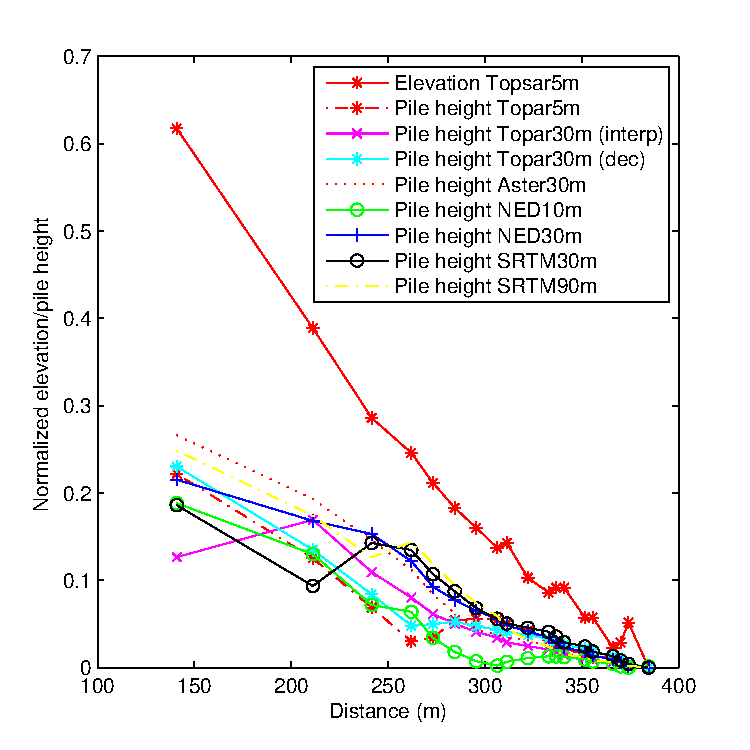
\includegraphics[width=8cm,height=9cm,keepaspectratio]{plots/low_all.pdf}\\
      (a)
    \end{tabular}
  \end{minipage}
  % \hfill
  \begin{minipage}{0.5\textwidth}
    \begin{tabular}{c}
      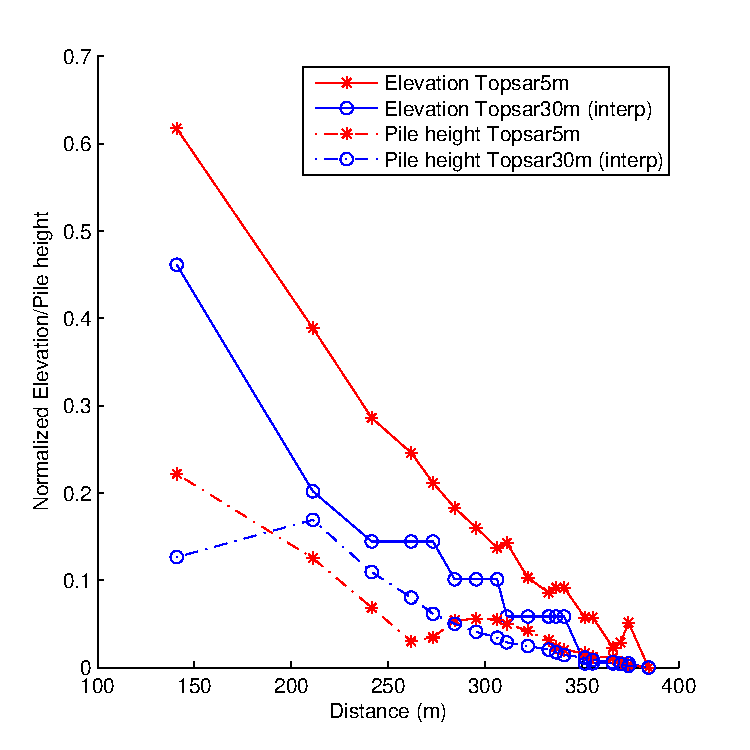
\includegraphics[width=8cm,height=9cm,keepaspectratio]{plots/low_T5_T30.pdf}\\
      (b)
    \end{tabular}
  \end{minipage}
  \begin{minipage}[b]{0.5\textwidth}
    \begin{tabular}{c}
      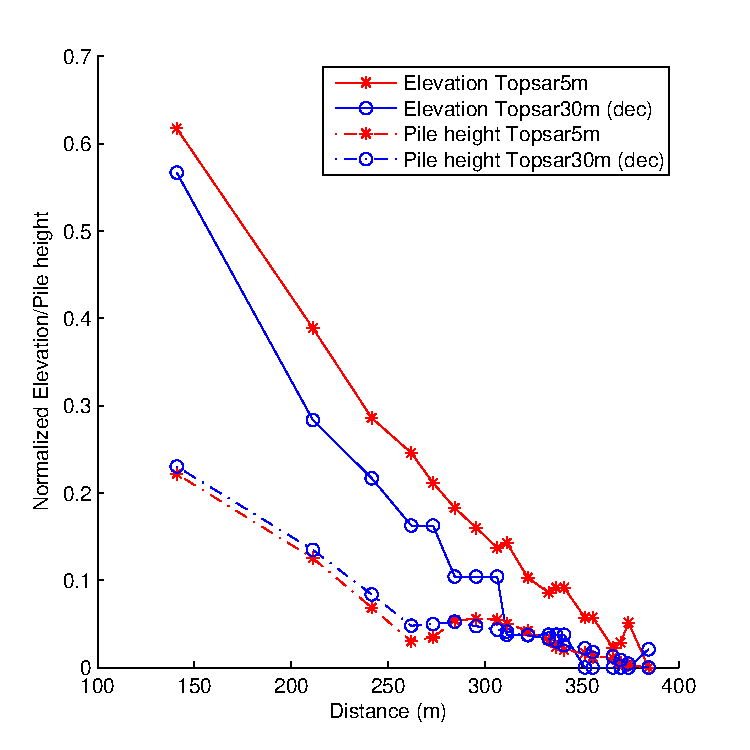
\includegraphics[width=8cm,height=9cm,keepaspectratio]{plots/low_T5_T30_3.pdf}\\
      (c)
    \end{tabular}
  \end{minipage}
  % \hfill
  \begin{minipage}{0.5\textwidth}
    \begin{tabular}{c}
      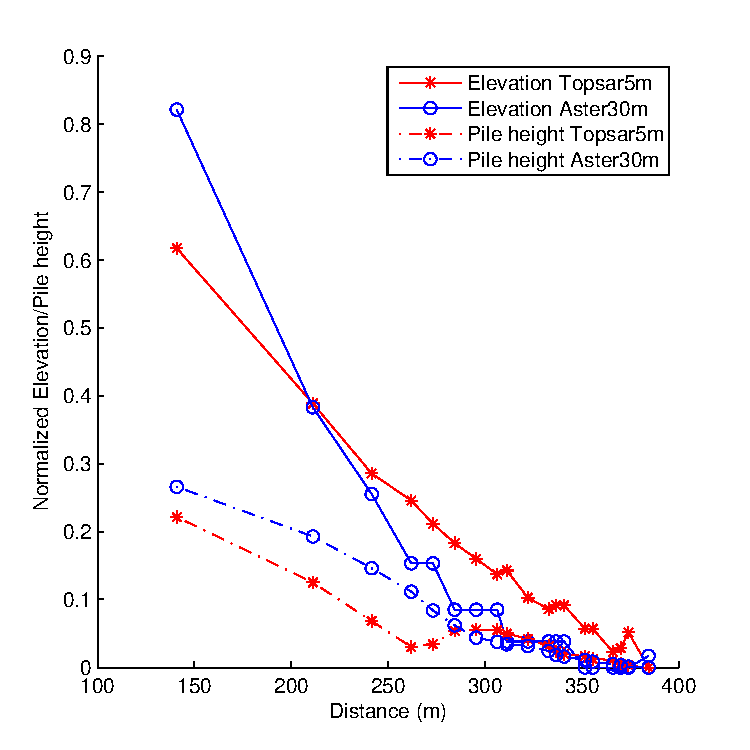
\includegraphics[width=8cm,height=9cm,keepaspectratio]{plots/low_T5_A30.pdf}\\
      (d)
    \end{tabular}
  \end{minipage}
  \caption{Normalized elevation and maximum pile height over time at the center line of the flow versus the distance -- low flow volume a) Topsar 5m normalized elevation vs normalized pile height of all output flow b) Topsar 5m vs Topsar 30m(interp) c) Topsar 5m vs Topsar 30m(dec) d) Topsar 5m vs Aster 30m }\label{fig10}
\end{figure}

\begin{figure}[H]
\ContinuedFloat 
  \begin{minipage}[b]{0.5\textwidth}
    \begin{tabular}{c}
      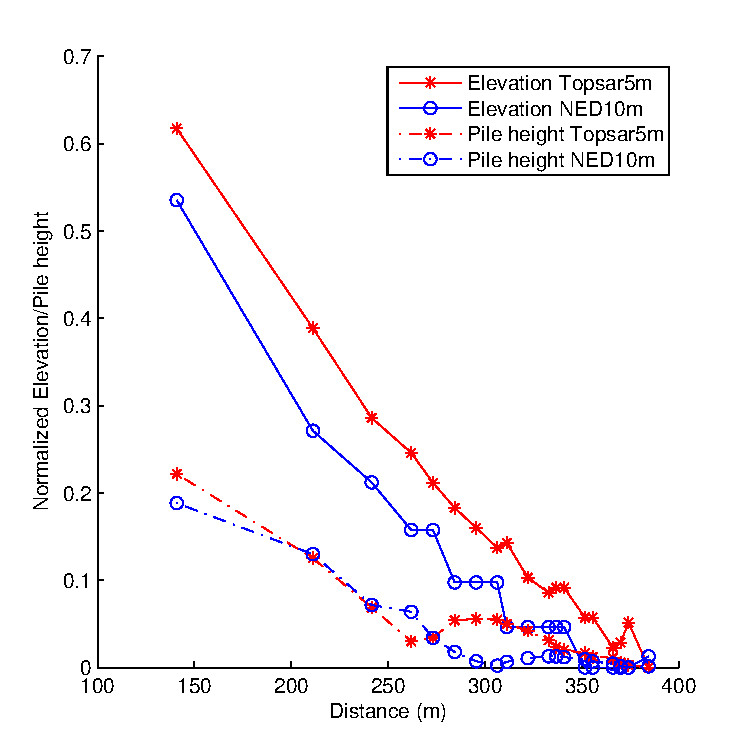
\includegraphics[width=8cm,height=9cm,keepaspectratio]{plots/low_T5_N10.pdf}\\
      (e)
    \end{tabular}
  \end{minipage}
  % \hfill
  \begin{minipage}{0.5\textwidth}
    \begin{tabular}{c}
      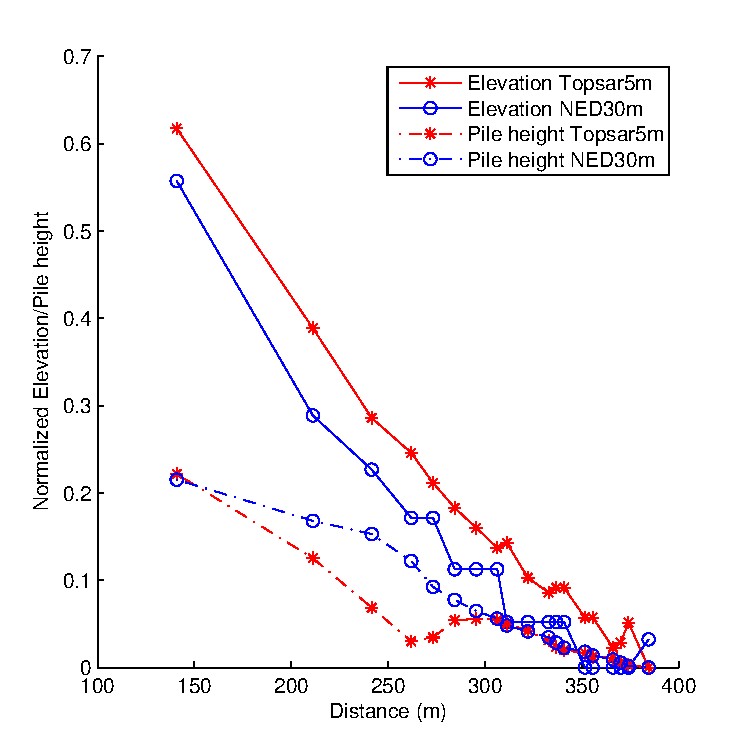
\includegraphics[width=8cm,height=9cm,keepaspectratio]{plots/low_T5_N30.pdf}\\
      (f)
    \end{tabular}
  \end{minipage}
  \begin{minipage}[b]{0.5\textwidth}
    \begin{tabular}{c}
      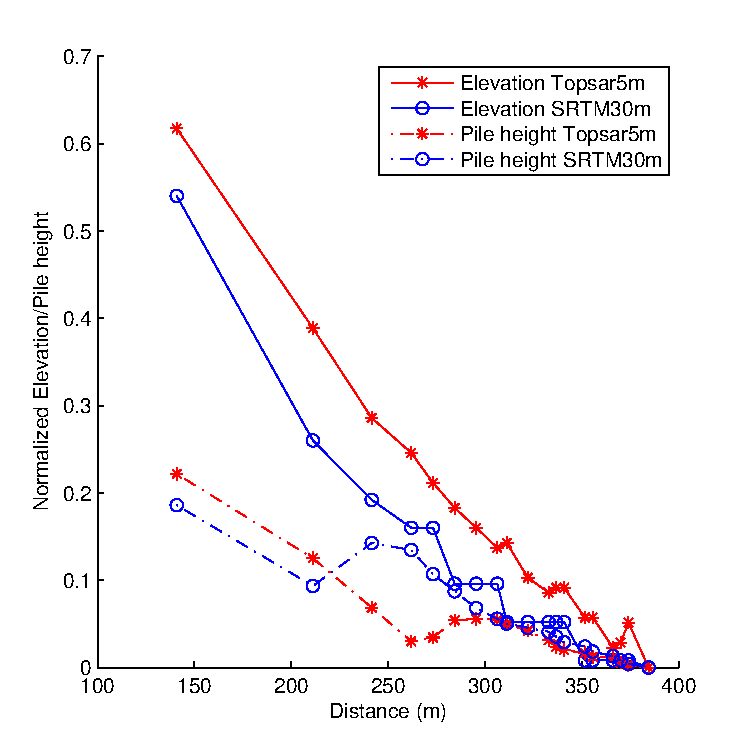
\includegraphics[width=8cm,height=9cm,keepaspectratio]{plots/low_T5_S30.pdf}\\
      (g)
    \end{tabular}
  \end{minipage}
  % \hfill
  \begin{minipage}{0.5\textwidth}
    \begin{tabular}{c}
      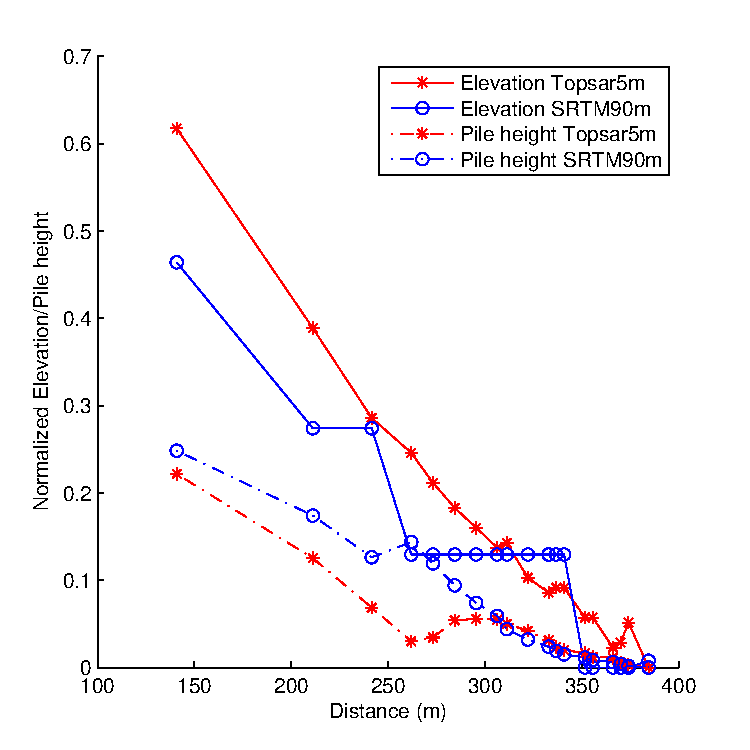
\includegraphics[width=8cm,height=9cm,keepaspectratio]{plots/low_T5_S90.pdf}\\
      (h)
    \end{tabular}
  \end{minipage}
   \caption{Normalized elevation and maximum pile height over time at the center line of the flow versus the distance -- low flow volume a) Topsar 5m vs NED 10m b) Topsar 5m vs NED 30m c) Topsar 5m vs SRTM 30m d) Topsar 5m vs SRTM 90m }\label{fig11}
\end{figure}

\begin{figure}[H]
  \begin{minipage}[b]{0.5\textwidth}
    \begin{tabular}{c}
      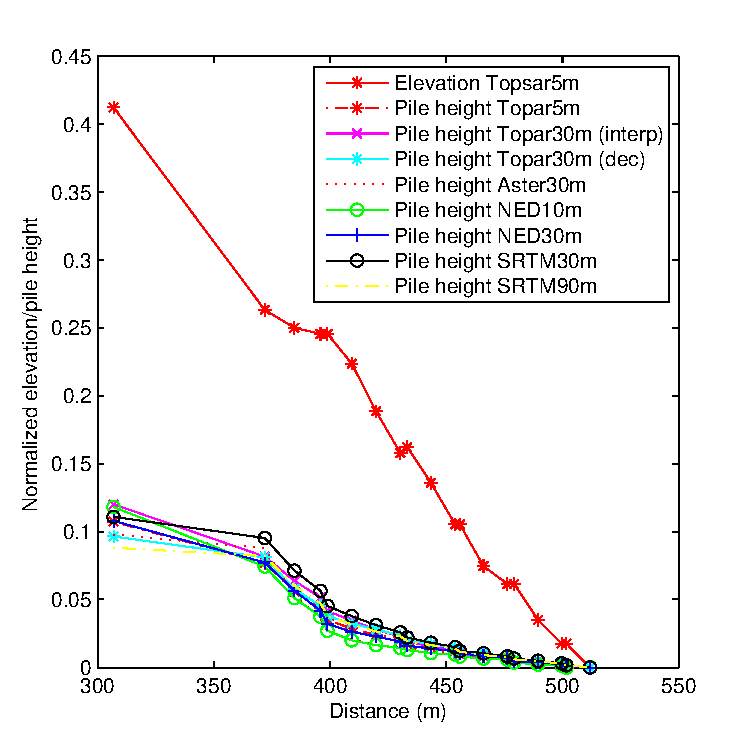
\includegraphics[width=8cm,height=9cm,keepaspectratio]{plots/high_all.pdf}\\
      (a)
    \end{tabular}
  \end{minipage}
  % \hfill
  \begin{minipage}{0.5\textwidth}
    \begin{tabular}{c}
      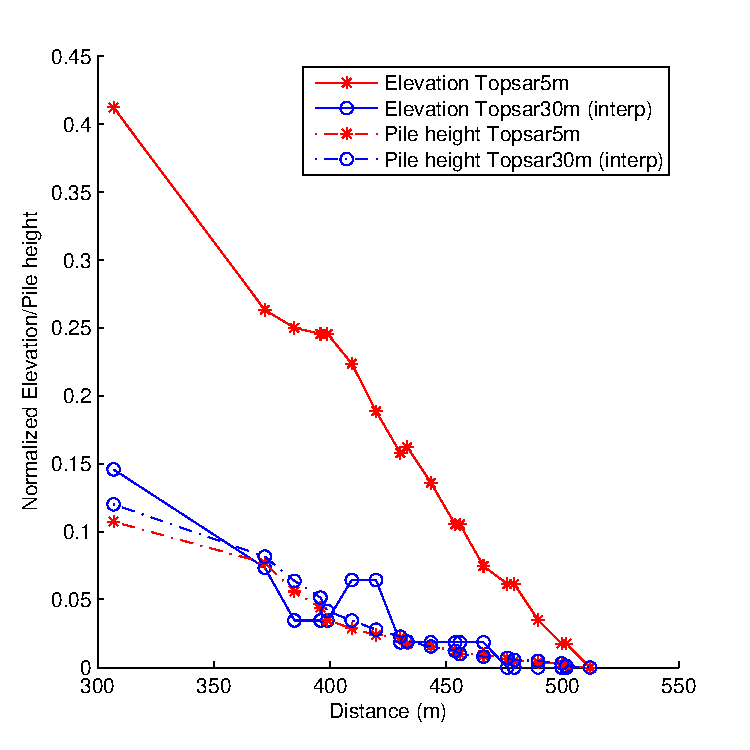
\includegraphics[width=8cm,height=9cm,keepaspectratio]{plots/high_T5_T30.pdf}\\
      (b)
    \end{tabular}
  \end{minipage}
  \begin{minipage}[b]{0.5\textwidth}
    \begin{tabular}{c}
      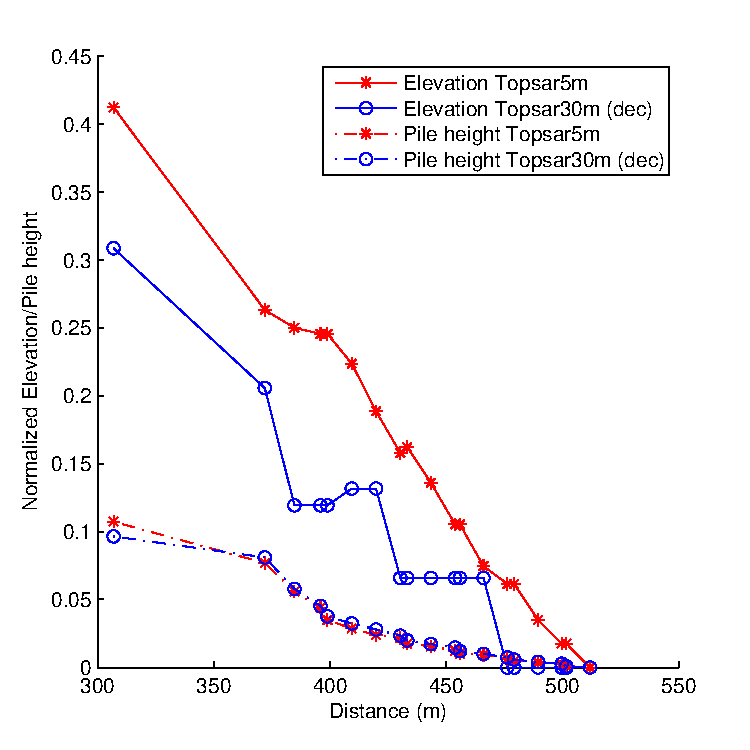
\includegraphics[width=8cm,height=9cm,keepaspectratio]{plots/high_T5_T30_3.pdf}\\
      (c)
    \end{tabular}
  \end{minipage}
  % \hfill
  \begin{minipage}{0.5\textwidth}
    \begin{tabular}{c}
      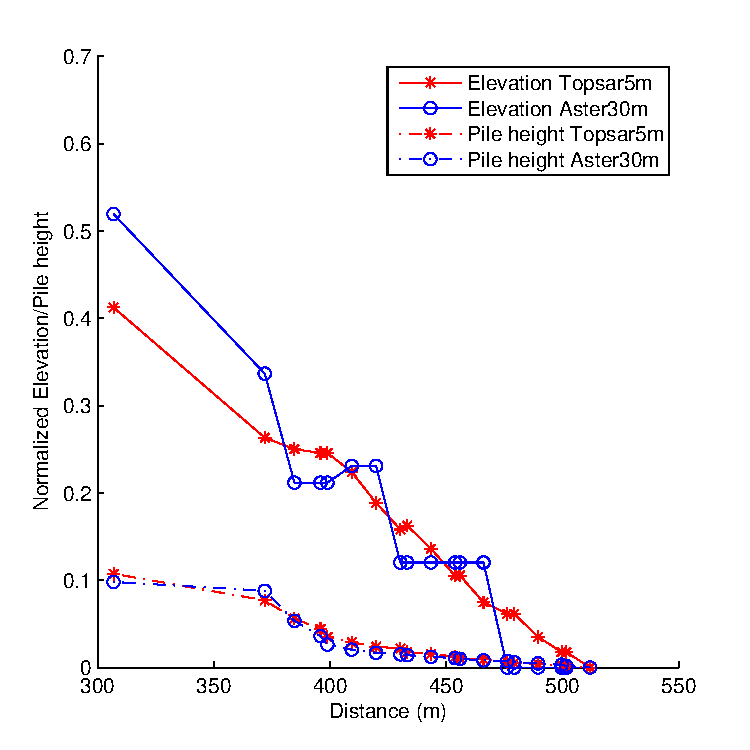
\includegraphics[width=8cm,height=9cm,keepaspectratio]{plots/high_T5_A30.pdf}\\
      (d)
    \end{tabular}
  \end{minipage}
   \caption{Normalized elevation and maximum pile height over time at the center line of the flow versus the distance -- high flow volume a) Topsar 5m normalized elevation vs normalized pile height of all output flow b) Topsar 5m vs Topsar 30m(interp) c) Topsar 5m vs Topsar 30m(dec) d) Topsar 5m vs Aster 30m }\label{fig12}
\end{figure}

\begin{figure}[H]
\ContinuedFloat 
  \begin{minipage}[b]{0.5\textwidth}
    \begin{tabular}{c}
      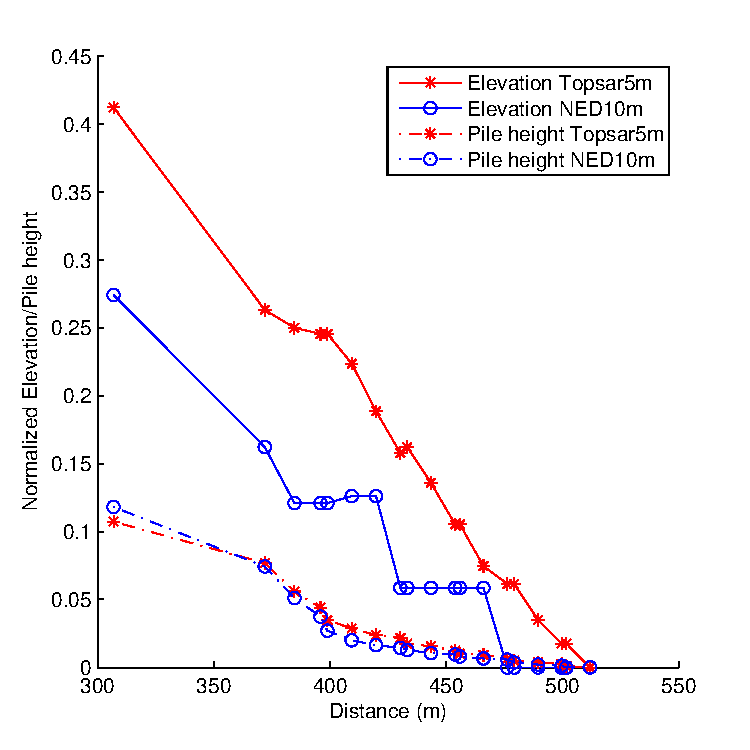
\includegraphics[width=8cm,height=9cm,keepaspectratio]{plots/high_T5_N10.pdf}\\
      (e)
    \end{tabular}
  \end{minipage}
  % \hfill
  \begin{minipage}{0.5\textwidth}
    \begin{tabular}{c}
      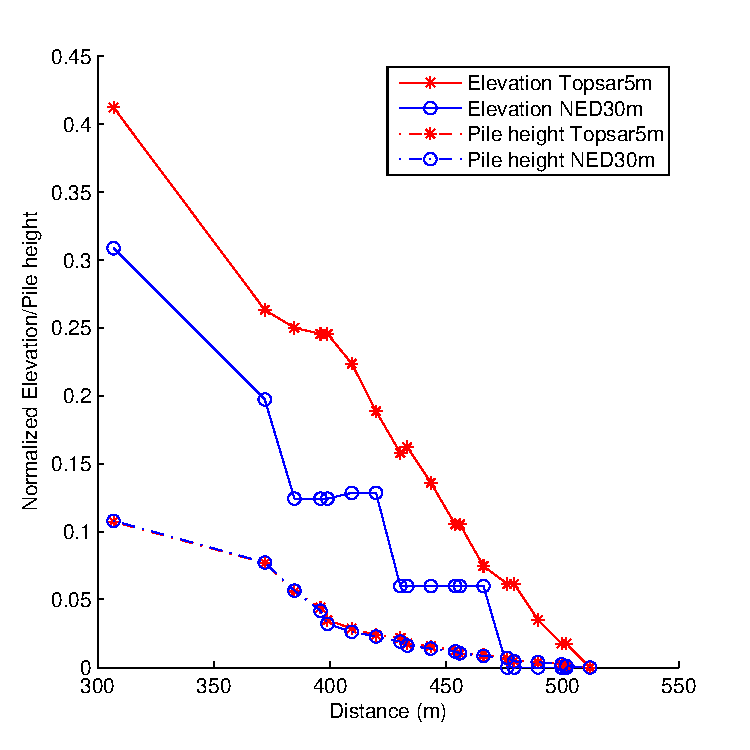
\includegraphics[width=8cm,height=9cm,keepaspectratio]{plots/high_T5_N30.pdf}\\
      (f)
    \end{tabular}
  \end{minipage}
  \begin{minipage}[b]{0.5\textwidth}
    \begin{tabular}{c}
      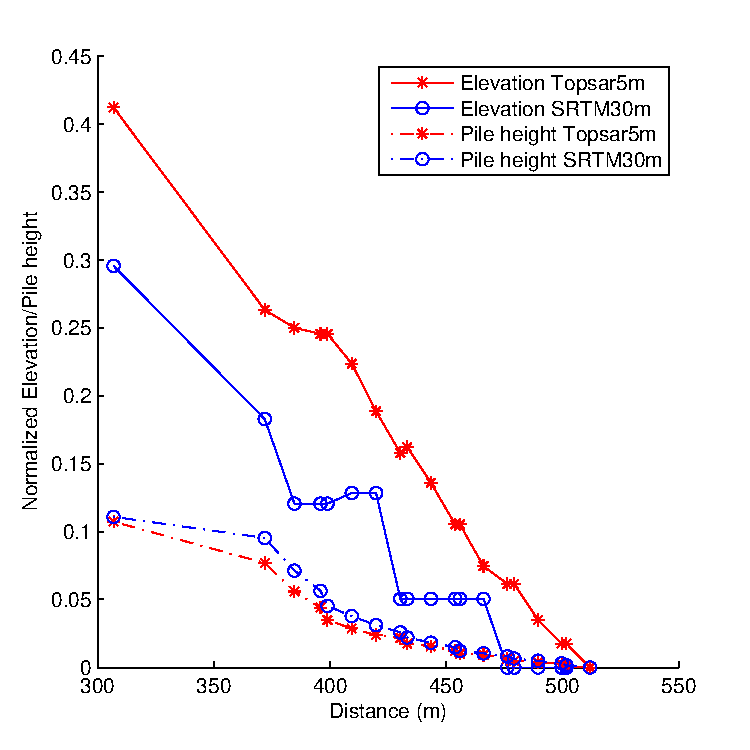
\includegraphics[width=8cm,height=9cm,keepaspectratio]{plots/high_T5_S30.pdf}\\
      (g)
    \end{tabular}
  \end{minipage}
  % \hfill
  \begin{minipage}{0.5\textwidth}
    \begin{tabular}{c}
      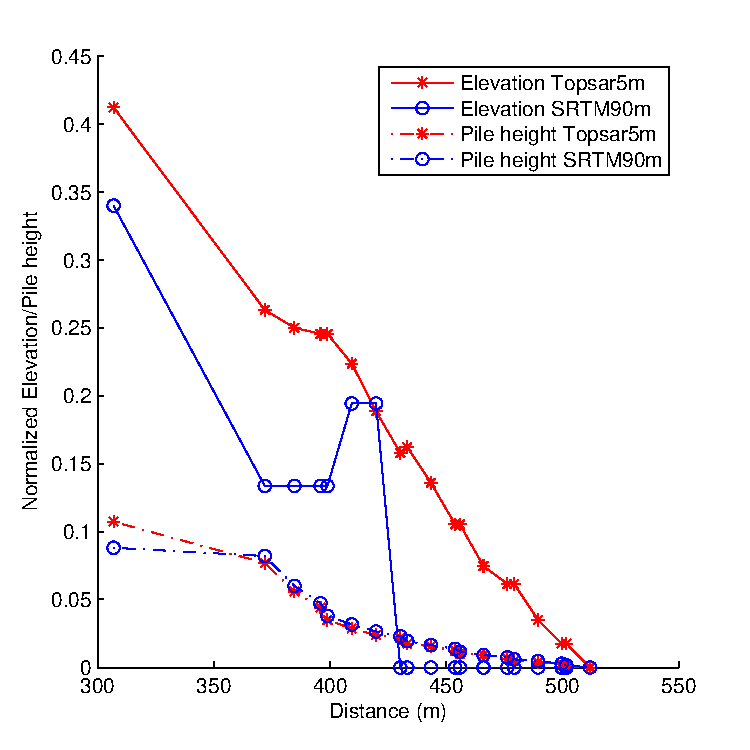
\includegraphics[width=8cm,height=9cm,keepaspectratio]{plots/high_T5_S90.pdf}\\
      (h)
    \end{tabular}
  \end{minipage}
  \caption{Normalized elevation and maximum pile height over time at the center line of the flow versus the distance -- high flow volume a) Topsar 5m vs NED 10m b) Topsar 5m vs NED 30m c) Topsar 5m vs SRTM 30m d) Topsar 5m vs SRTM 90m }\label{fig13}
\end{figure}

%\begin{figure}[H]
%  \begin{minipage}[b]{0.55\textwidth}
%    \begin{tabular}{c}
%      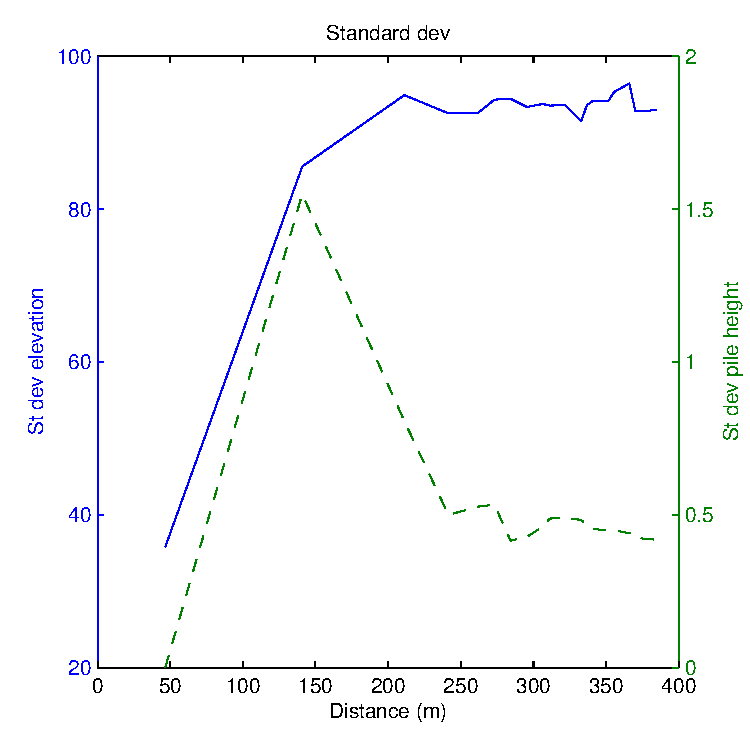
\includegraphics[width=8cm,height=9cm,keepaspectratio]{plots/low_st_dev.pdf}\\
%      (a)
%    \end{tabular}
%  \end{minipage}
%  % \hfill
%  \begin{minipage}{0.55\textwidth}
%    \begin{tabular}{c}
%      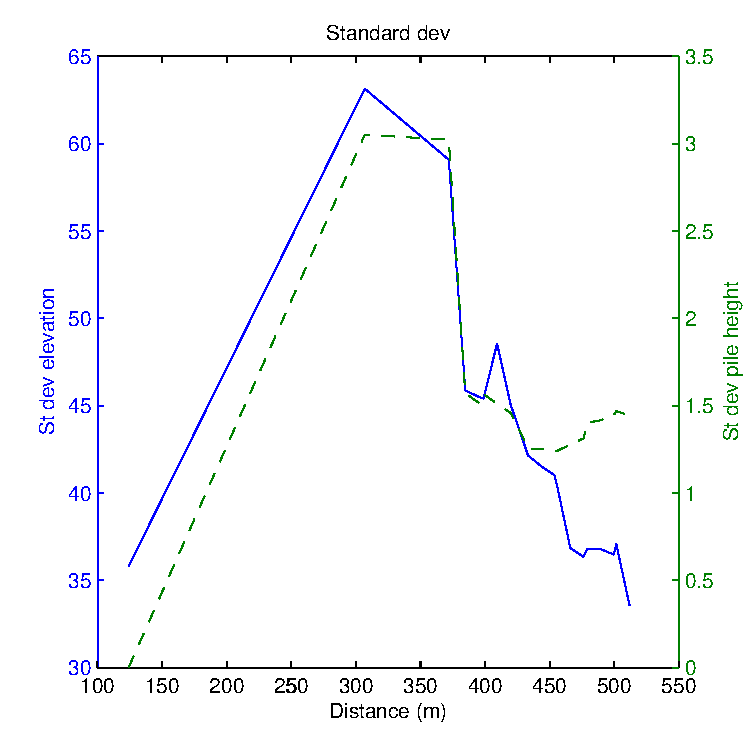
\includegraphics[width=8cm,height=9cm,keepaspectratio]{plots/high_st_dev.pdf}\\
%      (b)
%    \end{tabular}
%  \end{minipage}
%  \caption{Normalized standard deviation of the elevation and maximum pile height at center line of the flow a) low flow volume b)high flow volume}\label{fig14}
%\end{figure}


%\begin{figure}[H]
%  \begin{minipage}[b]{0.5\textwidth}
%    \begin{tabular}{c}
%      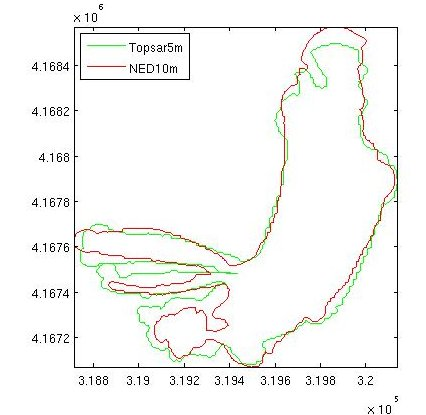
\includegraphics[width=5.5cm,height=7cm,keepaspectratio]{low_pics/TvNED10.jpg}\\
%      (a)
%    \end{tabular}
%  \end{minipage}
%  % \hfill
%  \begin{minipage}{0.5\textwidth}
%    \begin{tabular}{c}
%      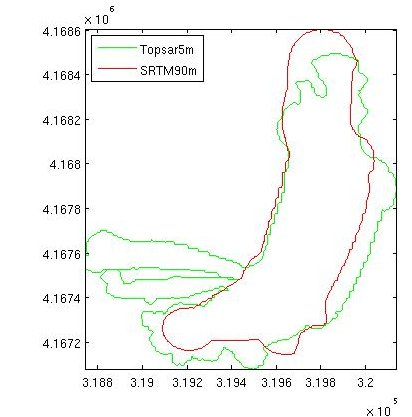
\includegraphics[width=5.5cm,height=7cm,keepaspectratio]{low_pics/TvsSRTM90.jpg}\\
%      (b)
%    \end{tabular}
%  \end{minipage}
%  % \caption{The footprint for low-volume flow (a) TOPSAR 5m vs NED
%  %   10m
%  %   (b)TOPSAR 5m vs SRTM 90m}\label{fig10}
%  % \end{figure}
%
%  % \begin{figure}[H]
%  %   \ContinuedFloat
%  \begin{minipage}[b]{0.5\textwidth}
%    \begin{tabular}{c}
%      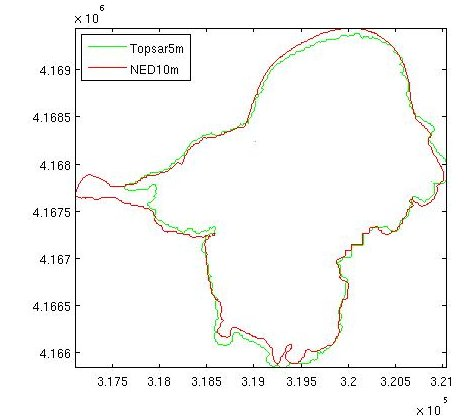
\includegraphics[width=6cm,height=7cm,keepaspectratio]{High_pics/TvNED10.jpg}\\
%      (c)
%    \end{tabular}
%  \end{minipage}
%  % \hfill
%  \begin{minipage}{0.5\textwidth}
%    \begin{tabular}{c}
%      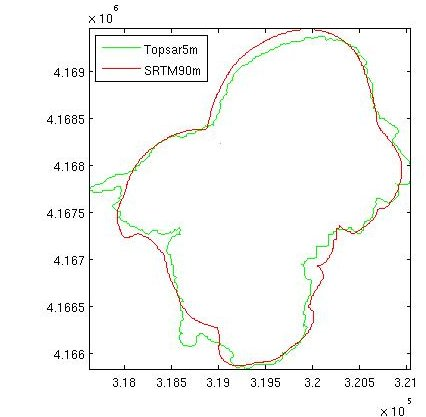
\includegraphics[width=6cm,height=7cm,keepaspectratio]{High_pics/TvSRTM90.jpg}\\
%      (d)
%    \end{tabular}
%  \end{minipage}
%  \caption{The footprint for the flow from Location 1 (a) TOPSAR5m vs
%    NED 10m low volume flow (b) TOPSAR 5m vs SRTM 90m low volume flow
%    (c) TOPSAR5m vs NED 10m high volume flow (d) TOPSAR 5m vs SRTM 90m
%    high volume flow)}\label{fig10}
%\end{figure}

\end{document}
